\documentclass{beamer}

\pdfmapfile{+sansmathaccent.map}


\mode<presentation>
{
  \usetheme{Warsaw} % or try Darmstadt, Madrid, Warsaw, Rochester, CambridgeUS, ...
  \usecolortheme{seahorse} % or try seahorse, beaver, crane, wolverine, ...
  \usefonttheme{serif}  % or try serif, structurebold, ...
  \setbeamertemplate{navigation symbols}{}
  \setbeamertemplate{caption}[numbered]
} 


%%%%%%%%%%%%%%%%%%%%%%%%%%%%
% itemize settings

\definecolor{mypink}{RGB}{255, 30, 80}
\definecolor{mydarkblue}{RGB}{60, 160, 255}
\definecolor{mydarkred}{RGB}{160, 30, 30}
\definecolor{mylightred}{RGB}{255, 150, 150}
\definecolor{myred}{RGB}{200, 110, 110}
\definecolor{myblackblue}{RGB}{40, 40, 120}
\definecolor{myblackred}{RGB}{120, 40, 40}
\definecolor{myblue}{RGB}{240, 240, 255}
\definecolor{mygreen}{RGB}{0, 200, 0}
\definecolor{mygreen2}{RGB}{205, 255, 200}
\definecolor{mygray}{gray}{0.8}
% \definecolor{mydarkgray}{gray}{0.4}
\definecolor{mydarkgray}{RGB}{80, 80, 160}

\setbeamertemplate{itemize items}[default]

\setbeamertemplate{itemize item}{\color{myblackred}$\blacksquare$}
\setbeamertemplate{itemize subitem}{\color{mydarkred}$\blacktriangleright$}
\setbeamertemplate{itemize subsubitem}{\color{mygray}$\blacksquare$}

\setbeamercolor{palette quaternary}{fg=white,bg=myred} %mydarkgray
\setbeamercolor{titlelike}{parent=palette quaternary}

\setbeamercolor{palette quaternary2}{fg=white,bg=mydarkred}%black myblue
\setbeamercolor{frametitle}{parent=palette quaternary2}

\setbeamerfont{frametitle}{size=\Large,series=\scshape}
\setbeamerfont{framesubtitle}{size=\normalsize,series=\upshape}





%%%%%%%%%%%%%%%%%%%%%%%%%%%%
% block settings

\setbeamercolor{block title}{bg=red!30,fg=black}

\setbeamercolor*{block title example}{bg=mygreen!40!white,fg=black}

\setbeamercolor*{block body example}{fg= black, bg= mygreen2}


%%%%%%%%%%%%%%%%%%%%%%%%%%%%
% URL settings
\hypersetup{
    colorlinks=true,
    linkcolor=blue,
    filecolor=blue,      
    urlcolor=blue,
}

%%%%%%%%%%%%%%%%%%%%%%%%%%

\renewcommand{\familydefault}{\rmdefault}

\usepackage{amsmath}
\usepackage{mathtools}
\usepackage{mathrsfs}


\usepackage{subcaption}

\usepackage{qrcode}

\DeclareMathOperator*{\argmin}{arg\,min}
\newcommand{\bo}[1] {\mathbf{#1}}

\newcommand{\dx}[1] {\dot{\mathbf{#1}}}
\newcommand{\ma}[4] {\begin{bmatrix}
    #1 & #2 \\ #3 & #4
    \end{bmatrix}}
\newcommand{\myvec}[2] {\begin{bmatrix}
    #1 \\ #2
    \end{bmatrix}}
\newcommand{\myvecT}[2] {\begin{bmatrix}
    #1 & #2
    \end{bmatrix}}
 
 \newcommand{\R}{\mathbb{R}} 
 \newcommand{\T}{^\top}     
    

\newcommand{\mydate}{Fall 2022}
\newcommand{\mygit}{\textcolor{blue}{\href{https://github.com/SergeiSa/Fundamentals-of-robotics-2022}{github.com/SergeiSa/Fundamentals-of-robotics-2022}}}


\newcommand{\bref}[2] {\textcolor{blue}{\href{#1}{#2}}}




%%%%%%%%%%%%%%%%%%%%%%%%%%%%
% code settings

\usepackage{listings}
\usepackage{color}
% \definecolor{mygreen}{rgb}{0,0.6,0}
% \definecolor{mygray}{rgb}{0.5,0.5,0.5}
\definecolor{mymauve}{rgb}{0.58,0,0.82}
\lstset{ 
  backgroundcolor=\color{white},   % choose the background color; you must add \usepackage{color} or \usepackage{xcolor}; should come as last argument
  basicstyle=\footnotesize,        % the size of the fonts that are used for the code
  breakatwhitespace=false,         % sets if automatic breaks should only happen at whitespace
  breaklines=true,                 % sets automatic line breaking
  captionpos=b,                    % sets the caption-position to bottom
  commentstyle=\color{mygreen},    % comment style
  deletekeywords={...},            % if you want to delete keywords from the given language
  escapeinside={\%*}{*)},          % if you want to add LaTeX within your code
  extendedchars=true,              % lets you use non-ASCII characters; for 8-bits encodings only, does not work with UTF-8
  firstnumber=0000,                % start line enumeration with line 0000
  frame=single,	                   % adds a frame around the code
  keepspaces=true,                 % keeps spaces in text, useful for keeping indentation of code (possibly needs columns=flexible)
  keywordstyle=\color{blue},       % keyword style
  language=Octave,                 % the language of the code
  morekeywords={*,...},            % if you want to add more keywords to the set
  numbers=left,                    % where to put the line-numbers; possible values are (none, left, right)
  numbersep=5pt,                   % how far the line-numbers are from the code
  numberstyle=\tiny\color{mygray}, % the style that is used for the line-numbers
  rulecolor=\color{black},         % if not set, the frame-color may be changed on line-breaks within not-black text (e.g. comments (green here))
  showspaces=false,                % show spaces everywhere adding particular underscores; it overrides 'showstringspaces'
  showstringspaces=false,          % underline spaces within strings only
  showtabs=false,                  % show tabs within strings adding particular underscores
  stepnumber=2,                    % the step between two line-numbers. If it's 1, each line will be numbered
  stringstyle=\color{mymauve},     % string literal style
  tabsize=2,	                   % sets default tabsize to 2 spaces
  title=\lstname                   % show the filename of files included with \lstinputlisting; also try caption instead of title
}


%%%%%%%%%%%%%%%%%%%%%%%%%%%%
% URL settings
\hypersetup{
    colorlinks=false,
    linkcolor=blue,
    filecolor=blue,      
    urlcolor=blue,
}

%%%%%%%%%%%%%%%%%%%%%%%%%%

%%%%%%%%%%%%%%%%%%%%%%%%%%%%
% tikz settings

\usepackage{tikz}
\tikzset{every picture/.style={line width=0.75pt}}


\title{Introduction, 2D linkages}
\subtitle{Fundamentals of Robotics, Lecture 1}
\author{by Sergei Savin}
\centering
\date{\mydate}



\begin{document}
\maketitle


%\begin{frame}{Content}
%
%%\begin{itemize}
%%\item Motivation
%%\item Ordinary differential equations
%%\item Linear differential equations
%%\item Changing n-th order ODE to a State-Space form
%%\item State-Space to ODE
%%\item Read more
%%\end{itemize}
%
%\end{frame}



\begin{frame}{What is Robotics?}
% \framesubtitle{O}
\begin{flushleft}

Since you chose to study Robotics, you likely have thought about what the word refers to. There are famous attempts to define it:

\begin{itemize}
	 \item Combination of mechanics, electronics, sensors and software.
	 \item Study of machines that make decisions based on acquired data (as opposed to automation of repetitive processes).
	 \item Science of making robots, which include industrial arms, quadrotors, automatic vacuum cleaners and walking robots - but does not include washing machines, airplanes and rockets. Are autonomous cars included?
\end{itemize}

I propose that we use the term when we find it practically useful: if it helps to describe something as a robot, as part of Robotics, as "doing Robotics" - do it; if there is better terminology - use the better one instead.

\end{flushleft}
\end{frame}



\begin{frame}{What is this course about?}
% \framesubtitle{Part 1}
\begin{flushleft}

There are aspects of "core" robotics that are so universally required that it is safe to assume you will need it. That includes understanding kinematics and dynamics of serial linkages (such as industrial arms) or single rigid bodies (such as drones, underwater robots, cars, delivery robots) and their combination (walking robots, mobile manipulators). 

\bigskip

This course is here to give you the prerequisite knowledge expected of a robotics graduate.

\end{flushleft}
\end{frame}



\begin{frame}{What is this course about?}
	% \framesubtitle{Part 1}
	\begin{flushleft}
		
		More concretely, we need to have a very good understanding of:
		
		\bigskip
		
		\begin{itemize}
			\item Forward kinematics
			\item Frame transformations
			\item Jacobians, null spaces, Relations between forces and joint torques, between Cartesian and joint velocities
			\item Inverse kinematics
			\item Dynamics
			\item Trajectory planning
			\item ...and more
		\end{itemize}
		
		Most of those are directly useful for mobile and industrial robotics, but frame transformation is also used in computer vision, while trajectory planning is at the core of autonomous vehicles, rockets, airplanes, etc.
		
	\end{flushleft}
\end{frame}





\begin{frame}{Terminology}
%\framesubtitle{1st order}
\begin{flushleft}

Let us remember some terminology from classical mechanics.

\bigskip

A \emph{point mass} is an object characterized by its position $\bo{r} \in \R^3$, velocity $\bo{v} \in \R^3$ and mass $m \in \R$.

\bigskip

\begin{example}
	If you model a satellite in orbit, you would likely describe it through its position and velocity which determine its orbit, and its mass that influences how much acceleration external forces (or thrusters) can produce.
\end{example}

\end{flushleft}
\end{frame}



\begin{frame}{Terminology}
	%\framesubtitle{1st order}
	\begin{flushleft}
		
		
		A \emph{rigid body} is an object characterized by its position $\bo{r} \in \R^3$ and orientation $\bo{T} \in SO(3)$, velocity of its center of mass $\bo{v} \in \R^3$ and angular velocity $\omega \in \R^3$, its mass $m$ and moment of inertia $\bo{I} \in \R^{3 \times 3}$.
		
		\bigskip
		
		\begin{example}
			If you model a drone, it is better to describe not just its position, but also its orientation - to know where it can and cannot fly next, to know where the camera is facing, etc. It is good to know not only mass but also moment of inertia, to understand how quickly it can turn.
		\end{example}
		
	\end{flushleft}
\end{frame}




\begin{frame}{Joints}
	%\framesubtitle{1st order}
	\begin{flushleft}
		
		A \emph{joint} is a constraint placed on a rigid body, restricting its movements. The joint type we will focus on is pin joint - think of it as a door hinge, or as a motor; it allows the body to rotate around the joint's axis, but nothing else:
		
	
		% TODO: \usepackage{graphicx} required
		\begin{figure}
			\centering
			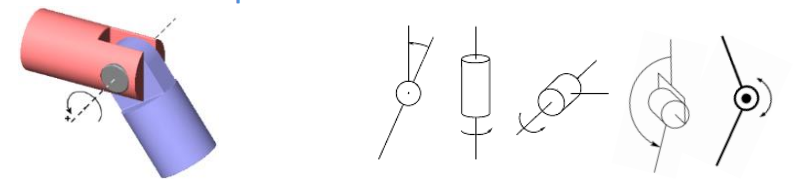
\includegraphics[width=0.7\linewidth]{PinJoints}
			\caption{Pin (revolute) joint - pictorial representation}
			\label{fig:pinjoints}
		\end{figure}
		
		
	\end{flushleft}
\end{frame}



\begin{frame}{Joints}
	%\framesubtitle{1st order}
	\begin{flushleft}
		
		Other joint types include:

		% TODO: \usepackage{graphicx} required
		\begin{figure}
			\centering
			\includegraphics[width=0.7\linewidth]{"Other joints"}
			\caption{Joints: (a), (b) - revolute, (c) - prizmatic, (d) - universal, (e) - spherical}
			\label{fig:other-joints}
		\end{figure}
		
		
	\end{flushleft}
\end{frame}




\begin{frame}{Joints}
	%\framesubtitle{1st order}
	\begin{flushleft}
		
		Industrial robots and walking robot mostly use revolute joints.	Big exception are orthogonal robots (like what you see in 3D printers), which use what we can describe as prismatic joints.
		
		\bigskip
		
		Everything that we will study in this course can be applied to all types of joints will small modifications; with that in mind we focus on pin joints.	
		
	\end{flushleft}
\end{frame}




\begin{frame}{Links}
	%\framesubtitle{1st order}
	\begin{flushleft}
		
		
		A rigid body attached to something (e.g. - to the ground) via a joint is called a \emph{link}. A link attached via a pin joint is characterized by its orientation $q \in \R$ and angular velocity $v \in \R$, its mass $m$ and moment of inertia $\bo{I} \in \R^{3 \times 3}$.
		
		\bigskip
		
		\begin{example}
			A pendulum can be described by its angle, angular velocity, its mass and moment of inertia.
		\end{example}
		
	\end{flushleft}
\end{frame}



\begin{frame}{One link robot}
	%\framesubtitle{1st order}
	\begin{flushleft}
		
		Let us consider a pendulum, described with angle $\varphi$ between its link and the vertical line. The length of the pendulum is given as $l$, point $\bo{r}_K$ is located at end of the pendulum.
		
		\bigskip
		
		\begin{columns}
			\begin{column}{0.5\textwidth}
				\tikzset{every picture/.style={line width=0.75pt}} %set default line width to 0.75pt        

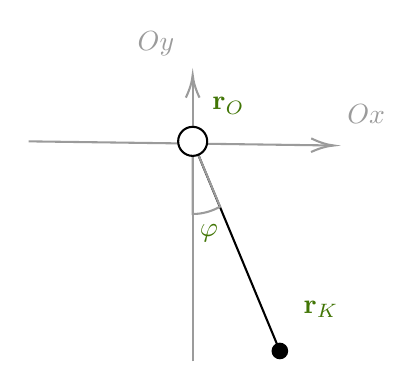
\begin{tikzpicture}[x=0.75pt,y=0.75pt,yscale=-1,xscale=1]
	%uncomment if require: \path (0,300); %set diagram left start at 0, and has height of 300
	
	%Straight Lines [id:da1514141660071826] 
	\draw [color={rgb, 255:red, 155; green, 155; blue, 155 }  ,draw opacity=1 ]   (171,175) -- (171,39) ;
	\draw [shift={(171,37)}, rotate = 90] [color={rgb, 255:red, 155; green, 155; blue, 155 }  ,draw opacity=1 ][line width=0.75]    (10.93,-3.29) .. controls (6.95,-1.4) and (3.31,-0.3) .. (0,0) .. controls (3.31,0.3) and (6.95,1.4) .. (10.93,3.29)   ;
	%Straight Lines [id:da8867696028247825] 
	\draw [color={rgb, 255:red, 155; green, 155; blue, 155 }  ,draw opacity=1 ]   (92,69) -- (237,70.97) ;
	\draw [shift={(239,71)}, rotate = 180.78] [color={rgb, 255:red, 155; green, 155; blue, 155 }  ,draw opacity=1 ][line width=0.75]    (10.93,-3.29) .. controls (6.95,-1.4) and (3.31,-0.3) .. (0,0) .. controls (3.31,0.3) and (6.95,1.4) .. (10.93,3.29)   ;
	%Straight Lines [id:da86988252841081] 
	\draw    (171,69) -- (213,170) ;
	%Shape: Circle [id:dp42453397326631825] 
	\draw  [fill={rgb, 255:red, 0; green, 0; blue, 0 }  ,fill opacity=1 ] (209.5,170) .. controls (209.5,168.07) and (211.07,166.5) .. (213,166.5) .. controls (214.93,166.5) and (216.5,168.07) .. (216.5,170) .. controls (216.5,171.93) and (214.93,173.5) .. (213,173.5) .. controls (211.07,173.5) and (209.5,171.93) .. (209.5,170) -- cycle ;
	%Shape: Pie [id:dp2450860928862184] 
	\draw  [color={rgb, 255:red, 155; green, 155; blue, 155 }  ,draw opacity=1 ] (184.19,100.45) .. controls (180.21,102.72) and (175.73,104) .. (171,104) -- (171,69) -- cycle ;
	%Shape: Circle [id:dp7741237432120269] 
	\draw  [fill={rgb, 255:red, 255; green, 255; blue, 255 }  ,fill opacity=1 ] (164,69) .. controls (164,65.13) and (167.13,62) .. (171,62) .. controls (174.87,62) and (178,65.13) .. (178,69) .. controls (178,72.87) and (174.87,76) .. (171,76) .. controls (167.13,76) and (164,72.87) .. (164,69) -- cycle ;
	
	% Text Node
	\draw (244,49.73) node [anchor=north west][inner sep=0.75pt]  [color={rgb, 255:red, 155; green, 155; blue, 155 }  ,opacity=1 ]  {$Ox$};
	% Text Node
	\draw (143,14.73) node [anchor=north west][inner sep=0.75pt]  [color={rgb, 255:red, 155; green, 155; blue, 155 }  ,opacity=1 ]  {$Oy$};
	% Text Node
	\draw (223,144.4) node [anchor=north west][inner sep=0.75pt]  [color={rgb, 255:red, 65; green, 117; blue, 5 }  ,opacity=1 ]  {$\bo{r}_{K}$};
	% Text Node
	\draw (179,46.4) node [anchor=north west][inner sep=0.75pt]  [color={rgb, 255:red, 65; green, 117; blue, 5 }  ,opacity=1 ]  {$\bo{r}_{O}$};
	% Text Node
	\draw (173,107.4) node [anchor=north west][inner sep=0.75pt]  [color={rgb, 255:red, 65; green, 117; blue, 5 }  ,opacity=1 ]  {$\varphi $};
	
	
\end{tikzpicture}

			\end{column}
			\begin{column}{0.5\textwidth}  %%<--- here
				
				Position of $\bo{r}_K$ is given as:
				
				\begin{equation}
					\bo{r}_K = \begin{bmatrix}
						l \sin (\varphi) \\ 
						-l \cos (\varphi) 
					\end{bmatrix}
				\end{equation}
				
				Differentiating the position we can find its velocity:
				
				\begin{equation}
					\dot{\bo{r}}_K = \begin{bmatrix}
						 l \dot \varphi \cos (\varphi) \\ 
						 l \dot \varphi \sin (\varphi) 
					\end{bmatrix}
				\end{equation}
				
				
			\end{column}
		\end{columns}
		
		
	\end{flushleft}
\end{frame}



\begin{frame}{One link robot}
	%\framesubtitle{1st order}
	\begin{flushleft}
		
		The forward kinematics can also be solved via rotation matrices:
		
		\begin{equation}
			\bo{r}_K = 
			\ma{\cos(\varphi)}{-\sin (\varphi)}{\sin (\varphi)}{\cos(\varphi)}
			\begin{bmatrix}
				0 \\ 
				-l 
			\end{bmatrix}
		=
			\begin{bmatrix}
				l \sin (\varphi) \\ 
				-l \cos (\varphi) 
			\end{bmatrix}
		\end{equation}
		
		
		
		
	\end{flushleft}
\end{frame}



\begin{frame}{Two link robot}
	%\framesubtitle{1st order}
	\begin{flushleft}
		
	
		\begin{columns}
			\begin{column}{0.4\textwidth}
				


\tikzset{every picture/.style={line width=0.75pt}} %set default line width to 0.75pt        

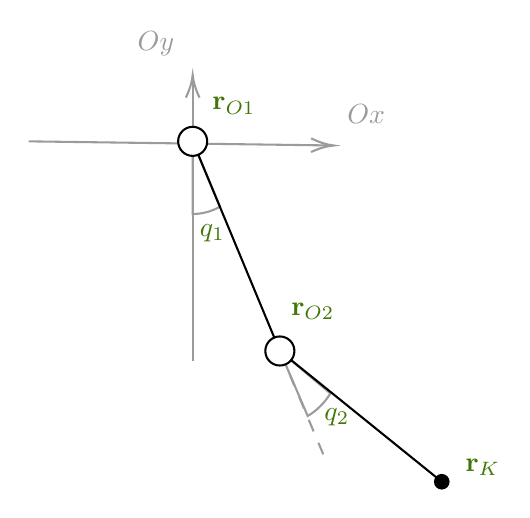
\begin{tikzpicture}[x=0.75pt,y=0.75pt,yscale=-1,xscale=1]
	%uncomment if require: \path (0,300); %set diagram left start at 0, and has height of 300
	
	%Shape: Pie [id:dp044024582329474704] 
	\draw  [color={rgb, 255:red, 155; green, 155; blue, 155 }  ,draw opacity=1 ] (237.35,190.45) .. controls (234.52,195.02) and (230.77,198.77) .. (226.42,201.31) -- (213,170) -- cycle ;
	%Shape: Pie [id:dp8327443137283965] 
	\draw  [color={rgb, 255:red, 155; green, 155; blue, 155 }  ,draw opacity=1 ] (184.19,100.45) .. controls (180.21,102.72) and (175.73,104) .. (171,104) -- (171,69) -- cycle ;
	%Straight Lines [id:da11981673752029831] 
	\draw [color={rgb, 255:red, 155; green, 155; blue, 155 }  ,draw opacity=1 ]   (171,175) -- (171,39) ;
	\draw [shift={(171,37)}, rotate = 90] [color={rgb, 255:red, 155; green, 155; blue, 155 }  ,draw opacity=1 ][line width=0.75]    (10.93,-3.29) .. controls (6.95,-1.4) and (3.31,-0.3) .. (0,0) .. controls (3.31,0.3) and (6.95,1.4) .. (10.93,3.29)   ;
	%Straight Lines [id:da4019711414513023] 
	\draw [color={rgb, 255:red, 155; green, 155; blue, 155 }  ,draw opacity=1 ]   (92,69) -- (237,70.97) ;
	\draw [shift={(239,71)}, rotate = 180.78] [color={rgb, 255:red, 155; green, 155; blue, 155 }  ,draw opacity=1 ][line width=0.75]    (10.93,-3.29) .. controls (6.95,-1.4) and (3.31,-0.3) .. (0,0) .. controls (3.31,0.3) and (6.95,1.4) .. (10.93,3.29)   ;
	%Straight Lines [id:da26868524985077347] 
	\draw    (171,69) -- (213,170) ;
	%Shape: Circle [id:dp05206742113524521] 
	\draw  [fill={rgb, 255:red, 0; green, 0; blue, 0 }  ,fill opacity=1 ] (287.75,233) .. controls (287.75,231.21) and (289.21,229.75) .. (291,229.75) .. controls (292.79,229.75) and (294.25,231.21) .. (294.25,233) .. controls (294.25,234.79) and (292.79,236.25) .. (291,236.25) .. controls (289.21,236.25) and (287.75,234.79) .. (287.75,233) -- cycle ;
	%Shape: Circle [id:dp009854061062177122] 
	\draw  [fill={rgb, 255:red, 255; green, 255; blue, 255 }  ,fill opacity=1 ] (164,69) .. controls (164,65.13) and (167.13,62) .. (171,62) .. controls (174.87,62) and (178,65.13) .. (178,69) .. controls (178,72.87) and (174.87,76) .. (171,76) .. controls (167.13,76) and (164,72.87) .. (164,69) -- cycle ;
	%Straight Lines [id:da271351498464834] 
	\draw    (213,170) -- (291,233) ;
	%Straight Lines [id:da15597835937675186] 
	\draw [color={rgb, 255:red, 155; green, 155; blue, 155 }  ,draw opacity=1 ] [dash pattern={on 4.5pt off 4.5pt}]  (213,170) -- (234,220) ;
	%Shape: Circle [id:dp48139269340211954] 
	\draw  [fill={rgb, 255:red, 255; green, 255; blue, 255 }  ,fill opacity=1 ] (206,170) .. controls (206,166.13) and (209.13,163) .. (213,163) .. controls (216.87,163) and (220,166.13) .. (220,170) .. controls (220,173.87) and (216.87,177) .. (213,177) .. controls (209.13,177) and (206,173.87) .. (206,170) -- cycle ;
	
	% Text Node
	\draw (244,49.73) node [anchor=north west][inner sep=0.75pt]  [color={rgb, 255:red, 155; green, 155; blue, 155 }  ,opacity=1 ]  {$Ox$};
	% Text Node
	\draw (143,14.73) node [anchor=north west][inner sep=0.75pt]  [color={rgb, 255:red, 155; green, 155; blue, 155 }  ,opacity=1 ]  {$Oy$};
	% Text Node
	\draw (301,220.4) node [anchor=north west][inner sep=0.75pt]  [color={rgb, 255:red, 65; green, 117; blue, 5 }  ,opacity=1 ]  {$\mathbf r_{K}$};
	% Text Node
	\draw (179,46.4) node [anchor=north west][inner sep=0.75pt]  [color={rgb, 255:red, 65; green, 117; blue, 5 }  ,opacity=1 ]  {$\mathbf r_{O1}$};
	% Text Node
	\draw (173,107.4) node [anchor=north west][inner sep=0.75pt]  [color={rgb, 255:red, 65; green, 117; blue, 5 }  ,opacity=1 ]  {$q_{1}$};
	% Text Node
	\draw (217,145.4) node [anchor=north west][inner sep=0.75pt]  [color={rgb, 255:red, 65; green, 117; blue, 5 }  ,opacity=1 ]  {$\mathbf r_{O2}$};
	% Text Node
	\draw (233,196.4) node [anchor=north west][inner sep=0.75pt]  [color={rgb, 255:red, 65; green, 117; blue, 5 }  ,opacity=1 ]  {$q_{2}$};
	
	
\end{tikzpicture}
			\end{column}
			\begin{column}{0.6\textwidth}  %%<--- here
				
					Let us consider a double-pendulum, described with angles $q_1$, $q_2$, with joints $O_1$, $O_2$ and \emph{end effector} $\bo{r}_K$, defined as before. The position of $K$ is given as:
				
					
					\begin{equation*}
						\bo{r}_K = \begin{bmatrix}
							l_1 \sin (q_1) + l_2 \sin (q_1+q_2) \\ 
							l_1 \cos (q_1) + l_2 \cos (q_1+q_2) 
						\end{bmatrix}
					\end{equation*}
				
			\end{column}
		\end{columns}
		
		
	\end{flushleft}
\end{frame}



\begin{frame}{Two link robot}
	%\framesubtitle{1st order}
	\begin{flushleft}
		
		Velocity of the end effector is found by differentiation:
		
				\begin{equation}
					\dot{\bo{r}}_K = 
					\begin{bmatrix}
						l_1 \dot q_1\cos (q_1) + l_2 (\dot q_1+\dot q_2) \cos (q_1+q_2) \\ 
					  - l_1 \dot q_1\sin (q_1)  - l_2 (\dot q_1+\dot q_2) \sin (q_1+q_2) 
					\end{bmatrix}
				\end{equation}
		
		If we introduce different variables $\varphi_1 = q_1$ and $\varphi_2 = q_1 + q_2$, the position and velocity of the end effector will take a simpler form:
		
		\begin{equation}
			\bo{r}_K = \begin{bmatrix}
				l_1 \sin (\varphi_1) + l_2 \sin (\varphi_2) \\ 
				l_1 \cos (\varphi_1) + l_2 \cos (\varphi_2) 
			\end{bmatrix}
		\end{equation}
		
		\begin{equation}
			\dot{\bo{r}}_K = 
			\begin{bmatrix}
				l_1 \dot \varphi_1\cos (\varphi_1) + l_2 \dot \varphi_2 \cos (\varphi_2) \\ 
			  - l_1 \dot \varphi_1\sin (\varphi_1)  - l_2 \dot \varphi_2 \sin (\varphi_2) 
			\end{bmatrix}
		\end{equation}
		
		\emph{The form of the kinematics depends on the choice of coordinates}. In this example $q_1$, $q_2$ are relative (joint) angles, and $\varphi_1$, $\varphi_2$ are absolute orientation.
		
	\end{flushleft}
\end{frame}



\begin{frame}{Two link robot}
	%\framesubtitle{1st order}
	\begin{flushleft}
		
		The forward kinematics can also be solved via rotation matrices:
		
		$$
			\bo{r}_K = 
			\ma{\cos(q_1)}{-\sin (q_1)}{\sin (q_1)}{\cos(q_1)}
			\begin{bmatrix}
				0 \\ 
				-l_1 
			\end{bmatrix}
		+$$
		$$+
		\ma{\cos(q_1+q_2)}{-\sin (q_1+q_2)}{\sin (q_1+q_2)}{\cos(q_1+q_2)}
		\begin{bmatrix}
			0 \\ 
			-l_2 
		\end{bmatrix}
			=$$
			$$
			=
			\begin{bmatrix}
				l_1 \dot q_1\cos (q_1) + l_2 (\dot q_1+\dot q_2) \cos (q_1+q_2) \\ 
				- l_1 \dot q_1\sin (q_1)  - l_2 (\dot q_1+\dot q_2) \sin (q_1+q_2) 
			\end{bmatrix}
		$$
		
		where:
		
		$$ \ma{\cos(q_1+q_2)}{-\sin (q_1+q_2)}{\sin (q_1+q_2)}{\cos(q_1+q_2)}  =$$
		$$=
		\ma{\cos(q_1)}{-\sin (q_1)}{\sin (q_1)}{\cos(q_1)}
		\ma{\cos(q_2)}{-\sin (q_2)}{\sin (q_2)}{\cos(q_2)}
		$$ 
		
		
		
		
		
	\end{flushleft}
\end{frame}



\begin{frame}{Angular velocity}
	%\framesubtitle{1st order}
	\begin{flushleft}
		
		Angular velocity of a rigid body is the rate of change of its orientation. In the last example, the orientation of the first link is given as $q_1$ and orientation of the second body - as $q_1 + q_2$. The rate of change of the orientation is found by differentiating these quantities:
		
		\begin{equation}
			\omega_1 = \dot q_1
		\end{equation}
		\begin{equation}
			\omega_2 = \dot q_1 + \dot q_2  
		\end{equation}
		
		This is so simple because we have an explicit expression defining orientation of the body; we will see next lecture that it is more difficult in 3D.
		
	\end{flushleft}
\end{frame}




\begin{frame}{Thank you!}
\centerline{Lecture slides are available via Moodle.}
\bigskip
\centerline{You can help improve these slides at:}
\centerline{\mygit}
\bigskip
\centerline{Check Moodle for additional links, videos, textbook suggestions.}
\bigskip

\centerline{\textcolor{black}{\qrcode[height=1.6in]{https://github.com/SergeiSa/Fundumentals-of-robotics-2022}}}

\end{frame}

\end{document}
